% Created 2019-06-22 Sat 19:52
% Intended LaTeX compiler: pdflatex
\documentclass[11pt]{article}
\usepackage[utf8]{inputenc}
\usepackage[T1]{fontenc}
\usepackage{graphicx}
\usepackage{grffile}
\usepackage{longtable}
\usepackage{wrapfig}
\usepackage{rotating}
\usepackage[normalem]{ulem}
\usepackage{amsmath}
\usepackage{textcomp}
\usepackage{amssymb}
\usepackage{capt-of}
\usepackage{hyperref}
\usepackage{minted}
\author{Nicolás Luarte}
\date{\today}
\title{Johans}
\hypersetup{
 pdfauthor={Nicolás Luarte},
 pdftitle={Johans},
 pdfkeywords={},
 pdfsubject={},
 pdfcreator={Emacs 25.2.2 (Org mode 9.2.3)}, 
 pdflang={English}}
\begin{document}

\maketitle
\tableofcontents

\section{Ciclos}
\label{sec:org26b83e3}
\subsection{Ciclo 1:}
\label{sec:org364ba4f}
\begin{center}
\begin{tabular}{lll}
\hline
Ejercicio & Protocolo & Bloque\\
\hline
Press banca de competencia & x1@8, 20\%, 4x5 & A\\
Press banca pies arriba & x1@8, 20\%, 2x5 & A\\
Press banca con mancuernas & x10@7, 8, 9, 2x10 & A\\
Skull crushers con mancuernas & x10@7, 8, 9, 2x10 & A\\
\hline
Press banca de competencia tempo 600 & x1@8, 20\%, 4x4 & B\\
Press banca agarre cerrado & x10@8, 10\%, 2x10 & B\\
Remos con mancuerna & x10@7, 8, 9, 2x10 & B\\
Press militar con mancuerna & x10@7, 8, 9, 2x10 & B\\
\hline
Peso muerto sumo desde bloque (justo abajo de la rodilla) & x10@100, 110, 120 & A\\
Peso muerto sumo hasta justo abajo de las rodillas & x10@90, 100, 110 & B\\
\hline
\end{tabular}
\end{center}

\section{Comentarios técnicos}
\label{sec:org1fec40b}
\subsection{11/06/2019 ciclo 1, bloque a:}
\label{sec:org00d15f4}
\subsubsection{Press banca de competencia:}
\label{sec:org841ef98}

\begin{enumerate}
\item Ajustar mejor el RPE, hubo ligero undershoot (un poquito mas bajo
de lo esperado)
\item La planta del pie debe estar completamente apoyada en el suelo
\item Para tomar la barra, rotar internamente las manos (un poco) de
manera tal que la barra descanse mas abajo en la palma
\item Aplicar "pausa activa", esto quiere decir, que la barra apenas toca
la primera fibra de tú polera, no debe hundirse en tú pecho.
\end{enumerate}

\subsubsection{Press banca pies arriba:}
\label{sec:org3050d2b}

\begin{enumerate}
\item Aplicar "pausa activa" y rotación de muñecas como especifique
arriba
\item Dejar los pies estirados
\item undershoot de RPE
\end{enumerate}

\subsubsection{Press banca con mancuernas:}
\label{sec:orgd1ebd10}

\begin{enumerate}
\item Undershoot de RPE
\end{enumerate}

\subsection{12/06/2019 ciclo 1, bloque b:}
\label{sec:org47f9a57}
\subsubsection{Press banca de competencia tempo 600}
\label{sec:org8e5c3b3}
\begin{enumerate}
\item Seguir trabajando el tocar la fibra de la polera, ahora agregando
el gesto de llevar el pecho hacia la barra, de manera activa
\item Ligeramente ir aumentando la rotación de la muñeca al tomar la
barra
\item Al momento de subir estás haciendo mucho "flare" con los codos, es
decir, los codos se te abren mucho, hasta cierto punto eso es
deseable, pero en este caso fue mucho, busca que al salir del pecho
los codos no se muevan tanto y permanezcan en su posición
\end{enumerate}
\subsubsection{Press banca agarre cerrado}
\label{sec:org8ed41b4}
\begin{enumerate}
\item Dado que este es un movimiento poco técnico, no hay muchas
correcciones que hacer, solo orientarlo a una conexión
mente-musculo mientras lo realizas, para obtener la mayor cantidad
de beneficio posible de esta variante, que tiene como foco
principal la hipertrofia
\end{enumerate}

\subsection{14/06/2019 ciclo 1, bloque a:}
\label{sec:org74e7f6c}
\subsubsection{Press banca de competencia}
\label{sec:org591c634}
\begin{enumerate}
\item Calcular mejor el RPE, aún lo estás estimando muy para abajo
\item Mantén mas tensión tocando el pecho, fuerza harto la clave de llevar el pecho a la barra
\item Antes de subir la barra del pecho se movió ligeramente hacia tú
cuello, eso puede ser por falta de tensión o simplemente perder la
atención, pero de todas maneras ponle harto ojo
\end{enumerate}
\subsubsection{Press banca pies arriba}
\label{sec:org9fd8b76}
\begin{enumerate}
\item Bien el RPE!
\item Trata de controlar los codos, evitando tanto flare, que queden un
poquito mas apegados a tus costillas
\end{enumerate}
\subsection{15/06/2019 ciclo 1, bloque b:}
\label{sec:org41e8397}
\subsubsection{Press banca de competencia tempo 600}
\label{sec:org45ec880}
\begin{enumerate}
\item Mantener el tempo hasta tocar el pecho, evitar que "rebote" o acelerar en los últimos centimetros
\item Trata de mantener un trayectoria en diagonal (recta) desde el pecho
hasta el rack, cualquier salida de esa línea imaginaria consideralo
cómo infeciencia, buscas siempre permanecer dentro de esa línea
\end{enumerate}
\subsubsection{Press banca agarre cerrado}
\label{sec:org8ed344b}
\begin{enumerate}
\item Nada que decir por ahora, esperaremos que tal va mientras van
subiendo los kg
\end{enumerate}
\subsection{18/06/2019 ciclo 1, bloque a:}
\label{sec:orgb23e766}
\subsubsection{Press banca de competencia}
\label{sec:org5a22ca3}
\begin{enumerate}
\item Concentrarse en tocar solo la fibra de la polera, nunca dejar de
hacer fuerza, intentar que la barra "flote" en el pecho
\item Al despegar no volver hundir la barra en el pecho
\end{enumerate}
\subsubsection{Press banca pies arriba}
\label{sec:org7eb8e2e}
\begin{enumerate}
\item Los mismos comentarios que para la banca de competencia
\end{enumerate}
\subsection{19/06/2019 ciclo 1, bloque b:}
\label{sec:org11080c0}
\subsubsection{Press banca de competencia tempo 600}
\label{sec:org3dbe695}
\begin{enumerate}
\item Harto mejor el tocar la fibra del pecho
\item Súper buena la sálida del pecho solo cuidar la posición de codos
\end{enumerate}
\subsubsection{Press banca agarre cerrado}
\label{sec:org4db9262}
\begin{enumerate}
\item Bien el RPE, la técnica está precisa
\end{enumerate}
\subsection{21/06/2019 ciclo 1, bloque a:}
\label{sec:orge89433e}
\subsubsection{Press banca de competencia}
\label{sec:org9ce7e19}
\begin{enumerate}
\item Ya estás dominando el RPE y el toque de pausa activa en el pecho
\item Ahora, el foco debiese estar en no lanzar los codos tan hacia
afuera, intenta mantenerlos un poco más cerrado. Cómo te mencioné
antes no es malo que los codoso queden afuera, de hecho puede ser
hasta beneficioso, lo que no queremos ver es un cambio de ángulo
drástico, ya que eso puede mover la barra
\end{enumerate}
\subsubsection{Press banca pies arriba}
\label{sec:org8548e0e}
\begin{enumerate}
\item Exactamente los mismos comentarios que para la banca de competencia
\end{enumerate}
\subsection{22/06/2019 ciclo 1, bloque b:}
\label{sec:orged33a06}
\subsubsection{Press banca de competencia tempo 600}
\label{sec:org572b4ac}
\begin{enumerate}
\item Ya tienes casi dominada la tocada en el pecho ahora lo que esta
faltando es la salida, cómo te he mencionado anteriormente, estás
tirando los codos muy para atrás así que quiero que pruebes tocar
ligeramente mas arriba en el pecho y partir con los codos un pelito
mas abiertos en la bajda
\item Aparte, antes de empezar con banca intenta meter unos remos
ligeros, 2x15 y sentir un ligero bombeo
\end{enumerate}
\subsubsection{Press banca agarre cerrado}
\label{sec:orgd261133}
\begin{enumerate}
\item Por ahora nada que decir
\end{enumerate}
\section{Registro de progreso}
\label{sec:orgd2c4d62}
\begin{center}
\label{tab:org838e368}
\begin{tabular}{lrrl}
Ejercicio & RPE & Peso & Fecha\\
\hline
Press banca de competencia & 7 & 92 & 11/06/2019\\
Press banca pies arriba & 7.5 & 85 & 11/06/2019\\
Press banca de competencia tempo 600 & 8 & 87.5 & 12/06/2019\\
Press banca agarre cerrado & 8 & 50 & 12/06/2019\\
Press banca de competencia & 7.5 & 95 & 14/06/2019\\
Press banca pies arriba & 8 & 87.5 & 14/06/2019\\
Press banca de competencia tempo 600 & 8 & 92.5 & 15/06/2019\\
Press banca agarre cerrado & 8 & 55 & 15/06/2019\\
Press banca de competencia & 8 & 95 & 18/06/2019\\
Press banca pies arriba & 8 & 87.5 & 18/06/2019\\
Press banca de competencia tempo 600 & 7.5 & 90 & 19/06/2019\\
Press banca agarre cerrado & 8 & 62 & 19/06/2019\\
Press banca de competencia & 8 & 95 & 21/06/2019\\
Press banca pies arriba & 8.5 & 87.5 & 21/06/2019\\
Press banca de competencia tempo 600 & 8.5 & 95 & 22/06/2019\\
Press banca agarre cerrado & 8 & 65 & 22/06/2019\\
 &  &  & \\
\end{tabular}
\end{center}
\begin{center}
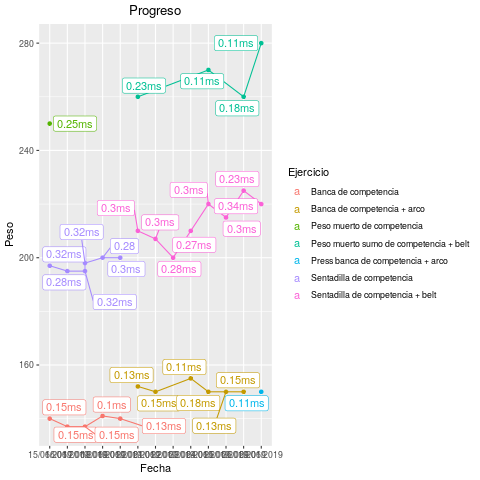
\includegraphics[width=.9\linewidth]{tmp.png}
\end{center}
\end{document}
